\input{preamble}
\usepackage{eurosym} %les euros
\newcommand{\C}{\mathcal{C}}

\begin{document}

\pagestyle{fancy}
\fancyhead[L]{Seconde}
\fancyhead[C]{\textbf{TD n°6 : fonctions carré, racine carrée, valeur absolue}}
\fancyhead[R]{\today}

Dans tout ce TD, on désigne pas $\Rp$ l'ensemble des réels \textbf{positifs}. $\Rp = [0, \infty[$.

\exe{}{
On donne :
\[ \dfrac{25}{16} = 1,5625 \quad ; \quad \dfrac{81}{64} = 1,265~625 \]
\textbf{Sans utiliser la calculatrice}, donner la valeur des carrés suivants :
\begin{multicols}{3}
\begin{enumerate}[label=(\alph*)]
\item $(0,8)^2$
\item $25^2 - 21^2$
\item $(1,25)^2$
\item $(1,125)^2$
\item $404^2$
\item $99^2$
\end{enumerate}
\end{multicols}
}{exe:1}{
\begin{enumerate}[label=(\alph*)]
\item $(0,8)^2 = \dfrac{8^2}{10^2} = 0,64$ ;
\item $25^2 - 21^2 = (25+21)(25-21) = 184$ ;
\item $1,25 \times 4 = 5$ donc $(1,25)^2 = \dfrac{25}{16} = 1,5625$ ;
\item $1,125 \times 8 = 9$ donc $(1,125)^2 = \dfrac{81}{64} = 1,265~625$ ;
\item $404^2 = (400+4)^2 = 400^2 + 2 \times 400 \times 4 + 4^2 = 163~216$ ;
\item $99^2 = (100-1)^2 = 100^2 - 2 \times 100 \times 1 + 1^2 = 9801$.
\end{enumerate}
}

\exe{}{
Pour chacune des questions ci-dessous, répondre par vrai ou faux \textbf{en justifiant}.
\begin{enumerate}
\item Pour tout $a, b \in \R$, on a $(a+b)^2 = a^2 + b^2$.
\item Pour $a, b \in \R$, si $a \leq b$ alors $a^2 \leq b^2$.
\item Pour $a, b \in \R$, si $0 \leq a \leq b$ alors $a^2 \leq b^2$.
\item Pour $a, b \in \R$, $\sqrt{a-b} = \sqrt{b-a}$.
\end{enumerate}
}{exe:2}{
\begin{enumerate}
\item Faux, prendre $a=1$ et $b=2$ par exemple.
\item Faux, prendre $a=-2$ et $b=1$ par exemple.
\item Vrai car $b^2 - a^2 = (b-a)(b+a)$ et $(b-a) \geq 0$ car $b \geq a$ et$(b+a) \geq 0$ car $a \geq 0$ et $b \geq 0$.
\item Faux, prendre $a=1$ et $b=0$ par exemple.
\end{enumerate}
}

\exe{}{
On donne :
\[ \sqrt{2} \approx 1,414~216 \quad ; \quad \sqrt{7} \approx 2,646 \quad ; \quad \sqrt{5} \approx 2,236 
\quad ; \quad  \sqrt{10} \approx 3,16 \]
\textbf{Sans utiliser la calculatrice}, donner une approximation des valeurs ci-dessous :
\begin{multicols}{2}
\begin{enumerate}[label=(\alph*)]
\item $\sqrt{20~000}$
\item $\sqrt{\frac74}$
\item $\sqrt{0,07}$
\item $\sqrt{\frac5{16}}$
\item $\sqrt{4^2+12^2}$
\item $\sqrt{100~000}$
\end{enumerate}
\end{multicols}
}{exe:3}{
\begin{enumerate}[label=(\alph*)]
\item $\sqrt{20~000} = \sqrt{2 \times 10~000} = \sqrt{2} \times 100 \approx 141,4216$ ;
\item $\sqrt{\dfrac74} = \dfrac{\sqrt{7}}{\sqrt{4}} \approx 1,323$ ;
\item $\sqrt{0,07} = \dfrac{\sqrt{7}}{\sqrt{100}} \approx 0,2646$ ;
\item $\sqrt{\dfrac5{16}} = \dfrac{\sqrt{5}}{\sqrt{16}} \approx 0,559$ ;
\item $\sqrt{4^2+12^2} = \sqrt{160} = \sqrt{16} \times \sqrt{10} = 12,64$ ;
\item $\sqrt{100~000} = \sqrt{10} \times \sqrt{10~000} \approx 316$ ;
\end{enumerate}
}

\exe{}{
	Écrire les nombres suivants sous la forme $a\sqrt{b}$ où $a\in\N$ est entier et $b\in\N$ est le 
	\textbf{plus petit entier naturel possible}.

	\begin{multicols}{3}
	\begin{enumerate}
		\item $\sqrt{12}$
		\item $\sqrt{150}$
		\item $5\sqrt{96}$
		\item $2\sqrt{300}$
		\item $\dfrac{12}{\sqrt{3}}$
		\item $\dfrac{18}{\sqrt{6}}$
		\item $\sqrt{125}$
	\end{enumerate}
	\end{multicols}
}{exe:4}{
	\begin{multicols}{2}
	\begin{enumerate}
		\item $\sqrt{12} = \sqrt{4\times3} = 2\sqrt3$
		\item $\sqrt{150} = \sqrt{25\times6} = 5\sqrt6$
		\item $5\sqrt{96} = \sqrt{16\times6} = 4\sqrt6$
		\item $2\sqrt{300} = 2\sqrt{3\times100} = 2\times10\sqrt3 = 20\sqrt3$
		\item $\dfrac{12}{\sqrt{3}} = \dfrac{12\sqrt3}{\sqrt3^2} = \dfrac{12\sqrt3}{3} = 4\sqrt3$
		\item $\dfrac{18}{\sqrt{6}} = \dfrac{18\sqrt6}{6} = 3\sqrt6$
		\item $\sqrt{125} = \sqrt{25\times5} = 5\sqrt5$
	\end{enumerate}
	\end{multicols}
}

\exe{}{
Tracer, dans le repère ci-dessous, une partie de la courbe représentative de la fonction valeur absolue.
\begin{center}
	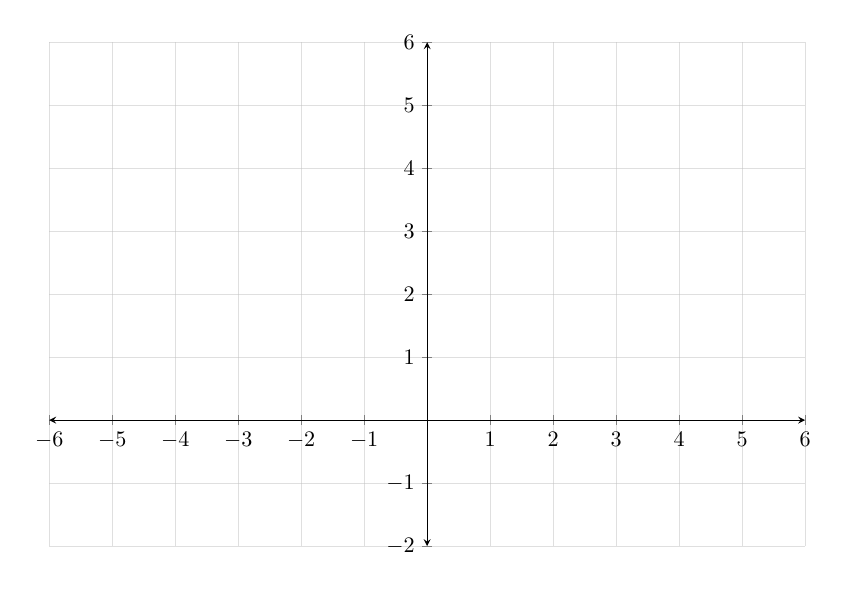
\begin{tikzpicture}[>=stealth, scale=.8]
		\begin{axis}[xmin = -6, xmax=6, ymin=-2, ymax=6, axis x line=middle, axis y line=middle, axis line style=<->, xlabel={}, ylabel={}, grid=both, grid style = {opacity=.5}, clip=false, xtick distance = 1, ytick distance=1, x=1cm, y=1cm]
		\end{axis}
	\end{tikzpicture}
\end{center}
}{exe:5}{
\begin{center}
	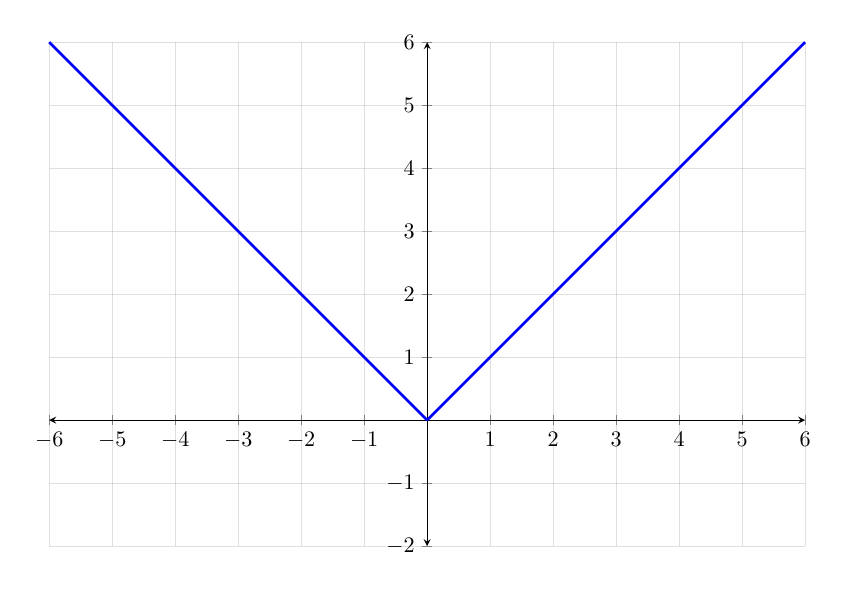
\begin{tikzpicture}[>=stealth, scale=.8]
		\begin{axis}[xmin = -6, xmax=6, ymin=-2, ymax=6, axis x line=middle, axis y line=middle, axis line style=<->, xlabel={}, ylabel={}, grid=both, grid style = {opacity=.5}, clip=false, xtick distance = 1, ytick distance=1, x=1cm, y=1cm]
		\addplot[blue, very thick, domain =0:6, samples=2] {x} ;
		\addplot[blue, very thick, domain =-6:0, samples=2] {-x} ;
		\end{axis}
	\end{tikzpicture}
\end{center}
}

\exe{}{
Pour chacun des cas ci-dessous, donner les valeurs possibles de $x$. Utiliser des intervalles si cela est pertinent.
	\begin{multicols}{2}
	\begin{enumerate}
		\item $\abs{x-20} = 10$
		\item $\abs{2x} < 20$
		\item $\abs{2x + 3} = 15$
		\item $\abs{2x - 1} > 7$  
	\end{enumerate}
	\end{multicols}
}{exe:6}{
	\begin{enumerate}
		\item $x = 30$ ou $x=10$ ;
		\item $x \in ]-10 ; 10 [$ ;
		\item $x = -9$ ou $x=6$ ;
		\item $x \in ]- \infty ; -3 [$ ou $x \in ]4; \infty[$.
	\end{enumerate}
}

\exe{, difficulty=1}{
Soit $f$ la fonction définie sur $\R$ par $f(x) = x^2 - a$, avec $a$ un nombre réel positif.
\begin{enumerate}
\item Donner l'expression littérale de $f(-x)$. Que peut-on dire de la fonction $f$ ?
\item On suppose qu'il existe $x_0 \in \Rp$ tel que $f(x_0) = 0$. Justifier que $f(-x_0)=0$.
\item Démontrer que $f(x) = (x-\sqrt{a})(x+\sqrt{a})$. En déduire la valeur de $\sqrt{a}$.
\item Application : on considère la fonction définie sur $\R$ par $f(x) = x^2 - 40$. On donne $f(6,35) = 0,3225$ et 
$f(6,25)=-0,9375$. Proposer un encadrement de $\sqrt{40}$. Préciser son amplitude.
\end{enumerate}
}{exe:7}{
\begin{enumerate}
\item $f(-x) = (-x)^2 - a = x^2 -a = f(x)$ donc $f$ est une fonction paire.
\item $f(-x_0)=f(x_0)=0$.
\item Il s'agit d'une identité remarquable. On en déduit que $f(\sqrt{a}) = 0$ donc $\sqrt{a} = x_0$ (car $\sqrt{a} \geq 0$). 
\item $f$ s'annule en $\sqrt{40}$. Par ailleurs, $f$ est croissante sur $\Rp$ 
(cf. exercice $\ref{exe:3}$, pour $0 \leq a \leq b$ on a $a^2 \leq b^2$ et donc $f(a) \leq f(b)$. 
On a donc $6,25 < \sqrt{40} < 6,35$. C'est un encadrement d'amplitude $10^{-1}$.
\end{enumerate}
}

\exe{, difficulty=1}{
On donne, ci-dessous, les représentations graphiques des fonctions définies sur $\Rp = [0 ; \infty[$ par :
\[ x \mapsto x \quad ; \quad x \mapsto x^2 \et x \mapsto \sqrt{x}. \]
La première fonction est appelée \og fonction identité \fg, les deux autres sont connues. \newline
\begin{center}
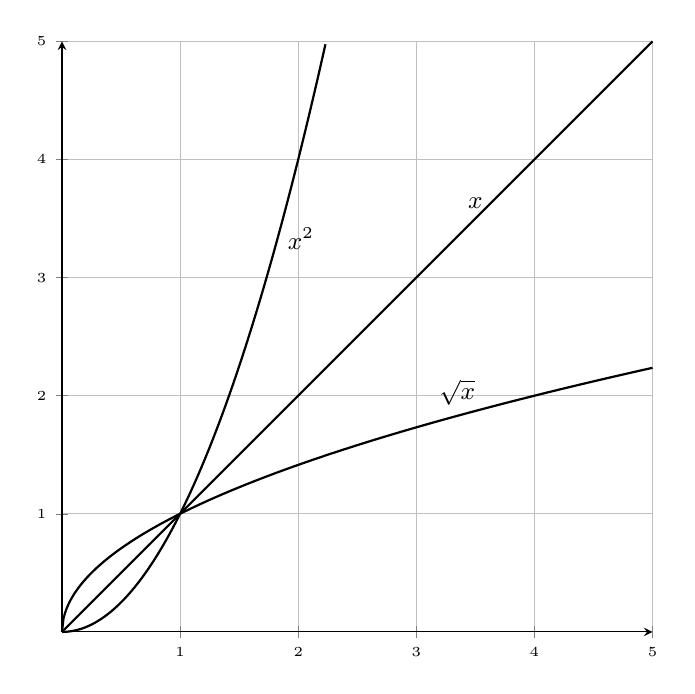
\begin{tikzpicture}[>=stealth, scale=1]
\begin{axis}%
    [
        grid=major,  
        x=15mm,
        y=15mm,
        xtick={0,...,5},   
        xmin=0,
        xmax=5,
        axis x line=middle,
        ytick={0,...,5},
        tick label style={font=\tiny},
        ymin=0,
        ymax=5,
        axis y line=middle,
        no markers,
        samples=100,
        domain=0:5,
        restrict y to domain=0:5,
        clip=false
    ]
    \addplot[thick,samples=400] (x,{x}) node[pos = 0.7, above, font=\small]{$x$};
    \addplot[thick,samples=400] (x,{x^2}) node[pos = 0.7, right, font=\small]{$x^2$};
    \addplot[thick,samples=400] (x,{x^(1/2)}) node[pos = 0.7, above, font=\small]{$\sqrt{x}$};
\end{axis} 
\end{tikzpicture}
\end{center}
Par lecture graphique, déterminer :
\begin{enumerate}
\item $x \in \Rp$ tel que $x=x^2=\sqrt{x}$ ;
\item $\{ x \in \Rp \tq x^2 < x \}$ ;
\item $\{ x \in \Rp \tq x^2 > x \}$ ;
\item $\{ x \in \Rp \tq \sqrt{x} < x \}$ ;
\item $\{ x \in \Rp \tq \sqrt{x} > x \}$.
\end{enumerate}
\textit{On donnera les résultats sous forme d'intervalle si cela est pertinent}. 
}{exe:8}{
\begin{enumerate}
\item $x=0$ ou $x=1$ ;
\item $x \in ]0 ; 1[$ ;
\item $x \in ]1 ; \infty [$ ;
\item $x \in ]1 ; \infty [$ ;
\item $x \in ]0 ; 1[$.
\end{enumerate}
Note : à savoir par coeur.
}

\newpage

\exe{, difficulty=1}{
Soit $g$ la fonction définie sur $\R$ par $g(x) = x^2 -10x +25$.
\begin{enumerate}
\item Montrer que l'on peut écrire $g(x) = (x-5)^2$.
\item Existe-t-il $x \in \R$ tel que $g(x) < 0$ ? Même question pour $g(x) = 0$.
\item Esquisser la représentation graphique de $\C_g$ dans le repère ci-dessous :
\begin{center}
	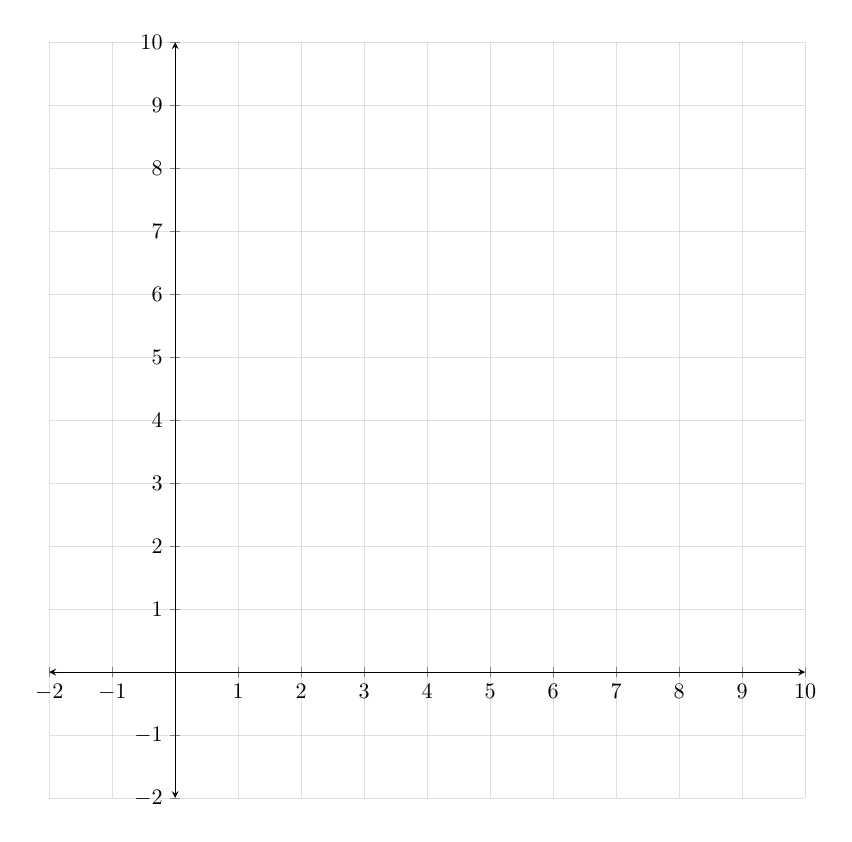
\begin{tikzpicture}[>=stealth, scale=.8]
		\begin{axis}[xmin = -2, xmax=10, ymin=-2, ymax=10, axis x line=middle, axis y line=middle, axis line style=<->, xlabel={}, ylabel={}, grid=both, grid style = {opacity=.5}, clip=false, xtick distance = 1, ytick distance=1, x=1cm, y=1cm]
		\end{axis}
	\end{tikzpicture}
\end{center}
\end{enumerate}
}{exe:9}{
\begin{enumerate}
\item Il s'agit d'une identité remarquable.
\item $g(x)=0$ pour $x=5$. Par contre $g(x)$ est un carré, donc toujours positif.
\item 
\begin{center}
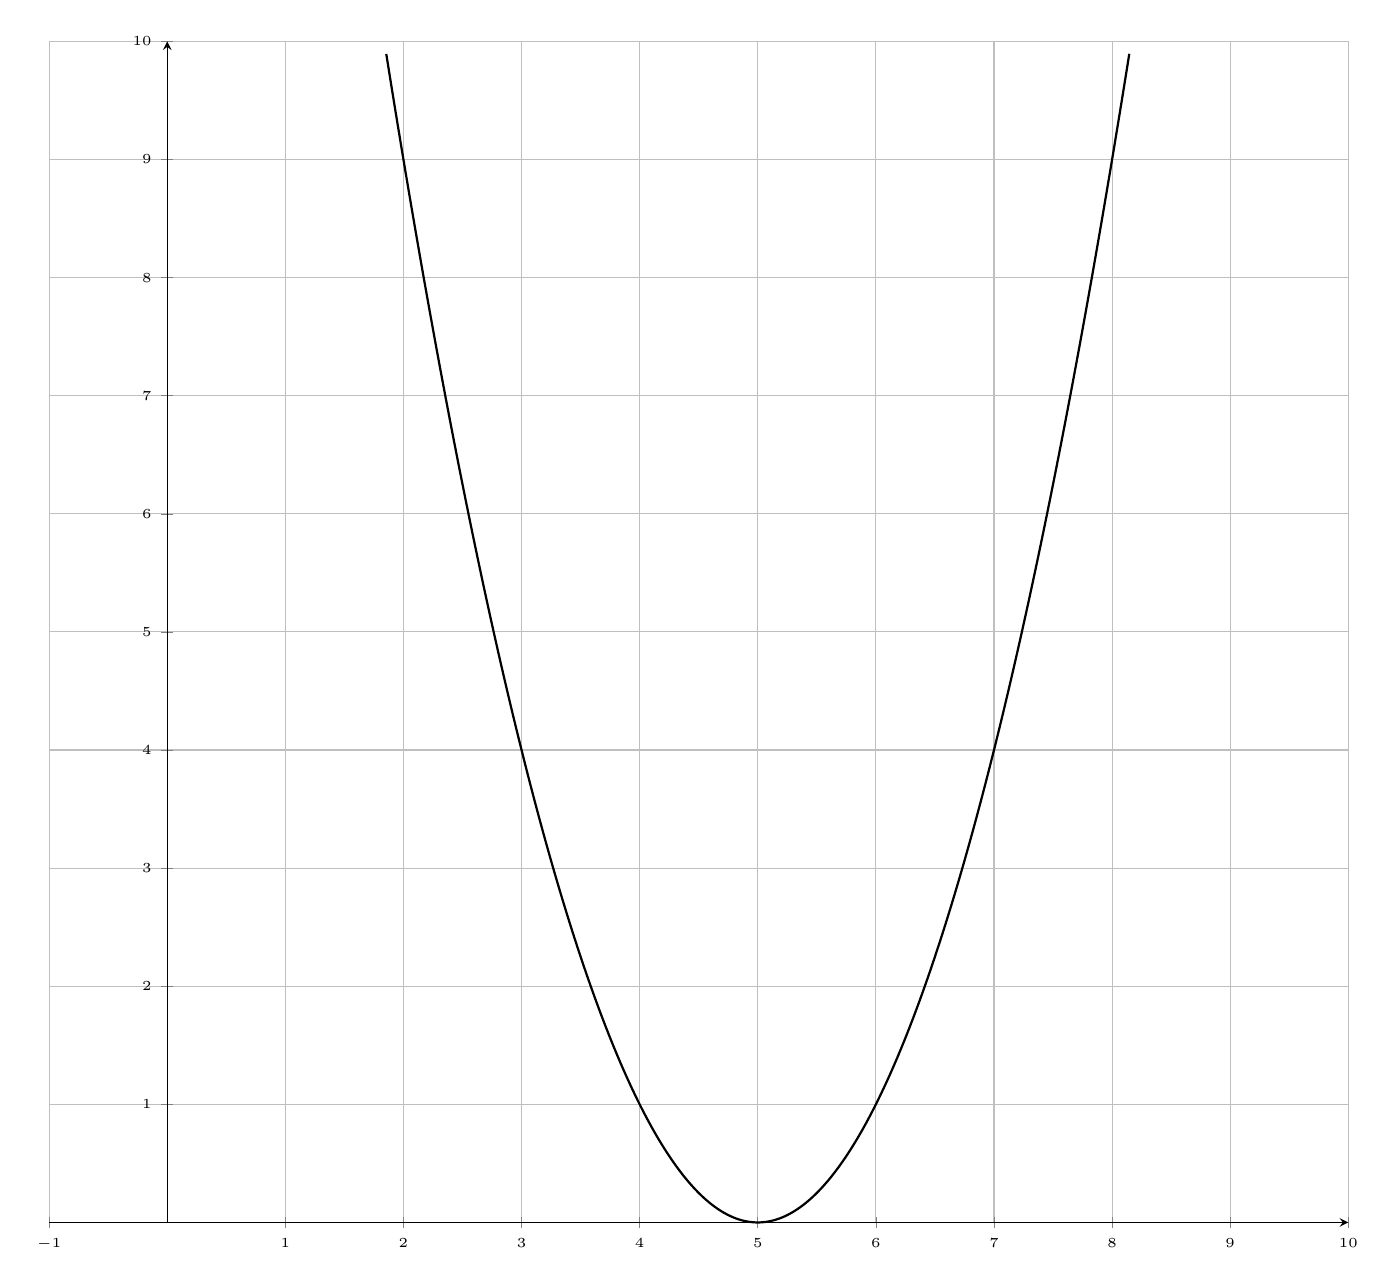
\begin{tikzpicture}[>=stealth, scale=1]
\begin{axis}
    [
        grid=major,  
        x=15mm,
        y=15mm,
        xtick={-1,...,10},   
        xmin=-1,
        xmax=10,
        axis x line=middle,
        ytick={-2,...,10},
        tick label style={font=\tiny},
        ymin=0,
        ymax=10,
        axis y line=middle,
        no markers,
        samples=100,
        domain=0:10,
        restrict y to domain=0:10,
        clip=false
    ]
    \addplot[thick,samples=400] (x,{(x-5)^2});

\end{axis} 
\end{tikzpicture}
\end{center}
\end{enumerate}
}

\exe{, difficulty=2}{
On note $n \in \N$, un entier naturel. 
\begin{enumerate}
\item Simplifier l'expression $(n+1)^2 - n^2$. Que remarquez-vous ?
\item On donne $426^2 = 181~476$. \textbf{Sans utiliser la calculatrice}, calculer $425^2$.
\end{enumerate}
}{exe:10}{
Exercice de recherche.
}

\exe{,difficulty = 2}{
On considère la fonction définie sur $\R$ par :
\[ \begin{array}{c c c c}
g : & \R & \to & \R \\
& x & \mapsto & x^2 -5x + 6
\end{array} \]
\begin{enumerate}
\item Montrer que $g(x) = (x-2)(x-3)$. \newline
\textit{Indication : développer l'expression $(x-2)(x-3)$}.
\item En déduire les éventuels antécédents de $0$ par $g$.
\item Donner un intervalle de $\R$ tel que $g(x) < 0$.
\item L'affirmation suivante est-elle vraie : \og si $x > 3$ alors $g(x) > 0$ \fg~? Justifier.
\item Même question pour l'affirmation : \og si $x < 2$ alors $g(x) > 0$ \fg.
\item Expliciter l'ensemble des réels $x \in \R$ tels que $g(x) > 0$.
\end{enumerate}
}{exe:11}{
Exercice de recherche.
}

\exe{, difficulty=2}{
Dans cet exercice, on utilisera le fait que la fonction \og racine carrée \fg~ est croissante sur $\Rp$.
\begin{enumerate}
\item Soient $a, b$ deux réels positifs tels que $a \leq b$. Sans la justifier, donne une relation d'ordre entre $\sqrt{a}$ et $\sqrt{b}$. 
\item Justifier que $1 \leq \sqrt{2} \leq 2$.
\item On donne $14^2 = 196$ et $15^2=225$. Justifier que $1,4 \leq \sqrt{2} \leq 1,5$. Quelle est l'amplitude de cet encadrement ?
\item Si on devait utiliser la même méthode pour obtenir un encadrement d'amplitude $10^{-2}$ de $\sqrt{2}$, 
quel nombre entier faudrait-il préalablement encadrer ?
Même question pour un encadrement d'amplitude $10^{-3}$.
\item En déduire une relation entre l'amplitude de l'encadrement et l'ordre de grandeur des nombres considérés.
\end{enumerate}
}{exe:12}{
Exercice de recherche.
}

%%%%%%%%%%%%

\newpage
\fancyhead[C]{\textbf{Solutions}}
\shipoutAnswer

\end{document}
